\begin{figure}[h]
    \centering
    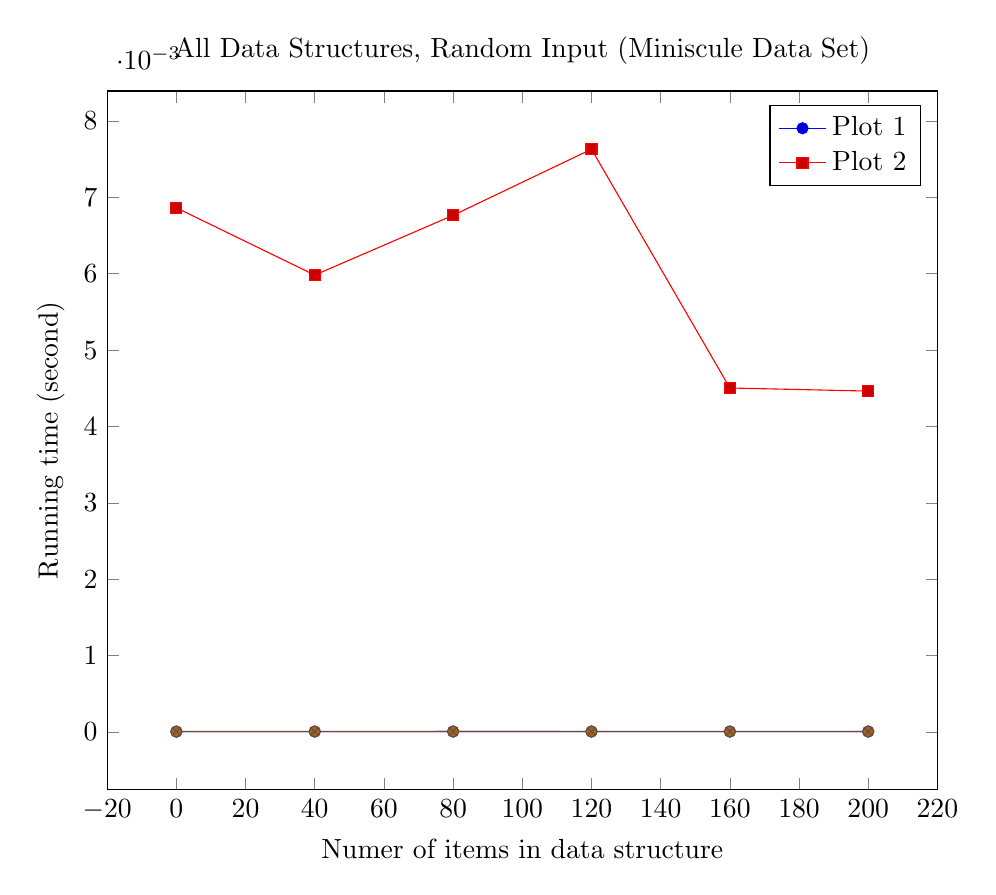
\begin{tikzpicture}
        \begin{axis}[
            xlabel={Numer of items in data structure},
            ylabel={Running time (second)},
            title={All Data Structures, Random Input (Miniscule Data Set)},
            width=\textwidth
        ]
		\addplot coordinates {
			(0, 3.7345741757208e-06)
			(40, 4.758570320676468e-06)
			(80, 4.9091579890522995e-06)
			(120, 5.210333325804048e-06)
			(160, 5.180215792128726e-06)
			(200, 5.752448931956901e-06)
		};
		\addplot coordinates {
			(0, 0.006862731810892031)
			(40, 0.00598218547883107)
			(80, 0.006764548651110936)
			(120, 0.0076304879793394065)
			(160, 0.0045036555156498185)
			(200, 0.00446314743285674)
		};
		\addplot coordinates {
			(0, 5.270568393100916e-06)
			(40, 5.15009825861057e-06)
			(80, 5.541626196148286e-06)
			(120, 4.698335253294772e-06)
			(160, 4.7886878544289855e-06)
			(200, 4.397159916535997e-06)
		};
        \legend{Plot 1, Plot 2}
        \end{axis}
    \end{tikzpicture}
    \caption{Average of 10 operations, benchmarked every 40, starting at 0. Median of 11 runs.}
\end{figure}